\subsection{Phase II\label{sec:phaseII}}

Phase II represents the evolution of Mosaic v1, our proof of concept. Phase II introduces two main components: a new active/passive liquidity model and a new and more complete set of features that deeply extend the functionality of Mosaic. Phase 2 allows to use different tokens on the source and destination layers, and also introduces the support for new chains such as Moonriver, Fantom, and Avalanche.

\subsubsection*{Active and passive liquidity}
In Mosaic v2 the user has the ability to provide liquidity on any layer and in exchange, besides the APY, he receives receipt tokens that can be integrated with other protocols (e.g: use them as collateral for loans). The user is also able to withdraw liquidity at any point he desires, our dynamic withdrawal fee will calculate the proportional rewards and the user will be credited with the right amount of tokens. Liquidity ca be also directly provided using ETH, and ETH can be transferred among the different layers. In addition to all these new possibilities, we introduce two types of liquidity for different profiles:

    \begin{itemize}
        \item \textbf{Passive liquidity:} In this type of liquidity providing, a more conservative user can obtain some rewards by providing liquidity in his desired layer. It can be understood as staking assets to yield some farm.  On the withdrawal, the user obtains the rewards and recovers the initial liquidity. Passive liquidity can only be withdrawn in the same token it was deposited. 
        
        \item \textbf{Active liquidity:} This liquidity providing model is intended for more knowledgeable and active users with an elevated risk appetite. By leveraging Composable SDK, they can run a dedicated bot to monitor the mempool and  the liquidity requirements of the transactions. If the liquidity of the destination layer is not enough, users can frontrun those transactions in order to gain greater rewards. Active liquidity is specified in number of blocks, and automatically becomes passive liquidity after that time. Active liquidity requires a flowing management but allows users to benefit from unbalanced networks to gain additional yield. Active liquidity can also be withdrawn in any token from any network.
    \end{itemize}
    
\subsubsection*{Cross Layer Function Calls}
Mosaic v2 not only supports value transfers, but also offers cross functions calls. The relayer can transfer the function call and its associated parameters from source to destination in a similar manner as value transfers. To handle calls and returns, it employs a \textit{MsgSender} contract on the source layer, which is in charge of abstracting the user and communicating with the relayer, and a \textit{MsgReceiverFactory} contract on the destination layer. \textit{MsgReceiverFactory} creates \textit{MsgReceiver} instances, which create a virtual identification of the user on the destination network, and interact with the desired protocol. All the interactions on the destination layer are done through the factory contract.

This general architecture, as shown on Fig.~(\ref{fig:crosscall}), allows users to call any protocol on any network and from any source. This elevates Mosaic v2 to a new level of unification, not only value is transferred, but also functionality is bridged together. 

\begin{figure}[H]
    \centering
    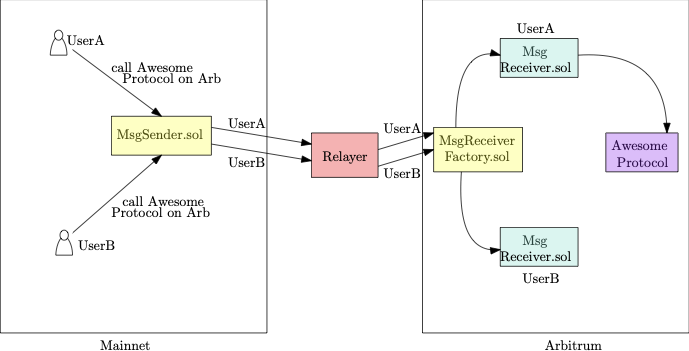
\includegraphics[width=0.9\textwidth]{images/mosaic/crosscalls.png}
    \caption{Cross layer function call architecture}
    \label{fig:crosscall}
\end{figure}


\subsubsection*{Other improvements}
In addition to the improvements already mentioned, phase II of the protocol presents the following and varied advances:

\begin{itemize}
    \item Transfer NFTs (ERC-721) between networks by using Ethereum research wrapper proposal \cite{WhyPropertiesb}.
    \item More secure and controlled vaults. Instead of a single \textit{MosaicVault}, everything is isolated in different and dedicated \textit{MosaicHoldings} smart contracts.
    \item Real time liquidity balancing. See Sec.~(\ref{section:lrs}) for more details.
    \item More efficient management of unused funds. Single or combined assets are used to yield farm, resulting in better and more competitive APY for Mosaic's liquidity providers.
\end{itemize}
